\documentclass{standalone}
\usepackage{tikz} % Import the tikz package
\usetikzlibrary{automata} % Import library for drawing automata
\usetikzlibrary{positioning} % ...positioning nodes
\usetikzlibrary{arrows} % ...customizing arrows
\tikzset{node distance=2.5cm,
    every state/.style={
        semithick,
        fill=gray!10},
    initial text={},
    double distance=2pt,
    every edge/.style={
        draw,
        ->,>=stealth',
        auto,
        semithick}}
\let\epsilon\varepsilon
\begin{document}
    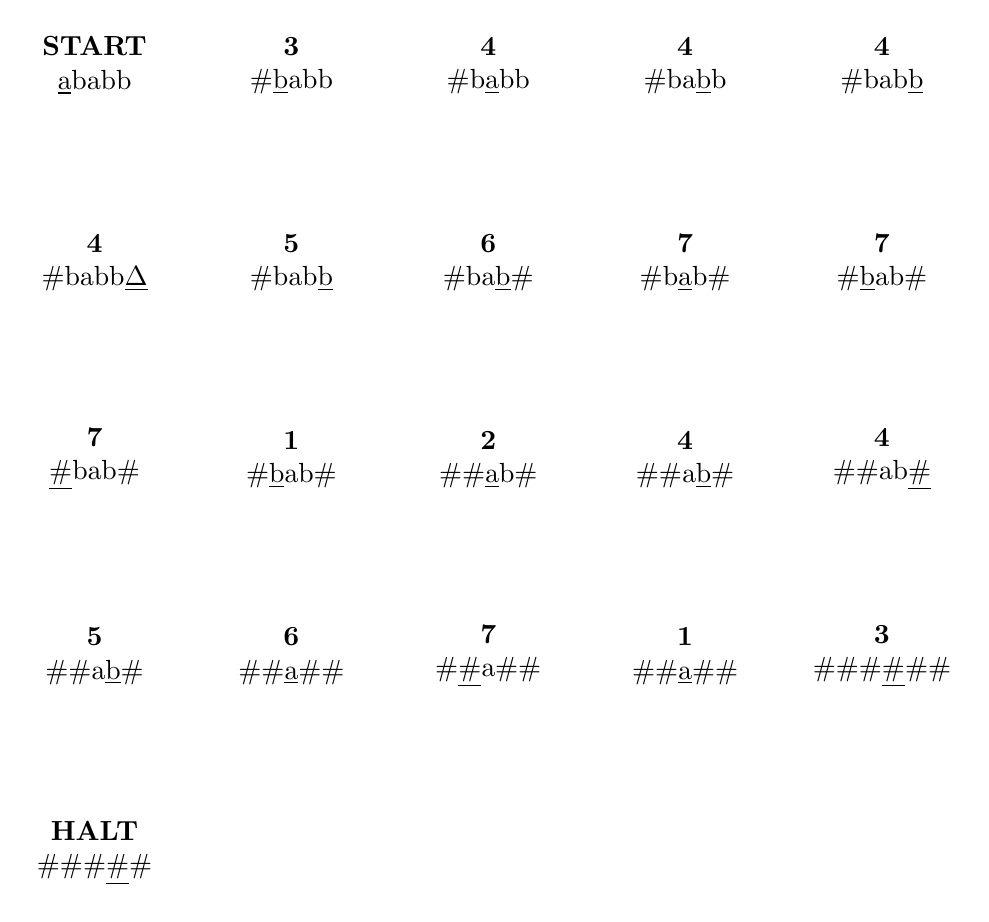
\begin{tikzpicture}
        
        \node[align=center] (1) {\textbf{START}\\\underline{a}babb};
        \node[align=center,right of=1] (2) {\textbf{3}\\\#\underline{b}abb};
        \node[align=center,right of=2] (3) {\textbf{4}\\\#b\underline{a}bb};
        \node[align=center,right of=3] (4) {\textbf{4}\\\#ba\underline{b}b};
        \node[align=center,right of=4] (5) {\textbf{4}\\\#bab\underline{b}};
        \node[align=center,below of=1] (6) {\textbf{4}\\\#babb\underline{$\Delta$}};
        \node[align=center,right of=6] (7) {\textbf{5}\\\#bab\underline{b}};
        \node[align=center,right of=7] (8) {\textbf{6}\\\#ba\underline{b}\#};
        \node[align=center,right of=8] (9) {\textbf{7}\\\#b\underline{a}b\#};
        \node[align=center,right of=9] (10) {\textbf{7}\\\#\underline{b}ab\#};
        \node[align=center,below of=6] (11) {\textbf{7}\\\underline{\#}bab\#};
        \node[align=center,right of=11] (12) {\textbf{1} \\\#\underline{b}ab\#};
        \node[align=center,right of=12] (13) {\textbf{2}\\\#\#\underline{a}b\#};
        \node[align=center,right of=13] (14) {\textbf{4}\\\#\#a\underline{b}\#};
        \node[align=center,right of=14] (15) {\textbf{4}\\\#\#ab\underline{\#}};
        \node[align=center,below of=11] (16) {\textbf{5}\\\#\#a\underline{b}\#};
        \node[align=center,right of=16] (17) {\textbf{6}\\\#\#\underline{a}\#\#};
        \node[align=center,right of=17] (18) {\textbf{7}\\\#\underline{\#}a\#\#};
        \node[align=center,right of=18] (19) {\textbf{1}\\\#\#\underline{a}\#\#};
        \node[align=center,right of=19] (20) {\textbf{3}\\\#\#\#\underline{\#}\#\#};
        \node[align=center,below of=16] (21) {\textbf{HALT}\\\#\#\#\underline{\#}\#};
    \end{tikzpicture}
\end{document}